% !TeX encoding = UTF-8
% !TeX spellcheck = en_US
% !TeX root = ../../../main.tex

\section{The framework}
\label{sec:framework}

The following section describes the framework which was developed during this thesis and how it could be used and configured. The framework was developed in two iterations. The first iteration was merely used during the initial experiments and resulted in a collection of \MATLAB scripts, barely useful for reuse but brought some insights into the possibilities of \MATLAB and for the next version of the framework. The second iteration was developed with having a future reuse and extendability in mind.

\subsection{First version}

\begin{wrapfigure}{r}{0.4\textwidth}
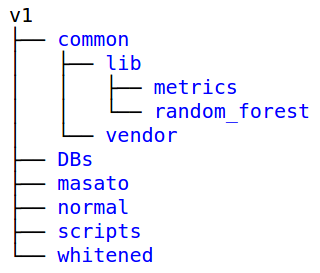
\includegraphics[width=\textwidth]{content/pictures/v1_dirs.png}
\caption{Framework v1 Directory layout}
\label{fig:framework_v1_dirs}
\end{wrapfigure}

The first version of the framework has its primary focus on the experiments involving different feature algorithms and the general investigation of the basic codebook performance. The main directory for the implemented \MATLAB scripts is the \textit{common} folder. It contains 16 files which are responsible for the extraction of features, clustering with k-Means and \ac{GMM}, generation of codebooks and visualization of the codebook comparisons. These scripts share and use in total 57 functions which resides inside the \textit{common/lib} folder to accomplish their work. As the experiments in this stage were done with \ac{HOG} and \ac{WHOG} in parallel, the folders \textit{normal} and \textit{whitened} respectively contain independent settings and scripts which require a different handling based on the used feature backend. The \textit{scripts} folder contain some shell and utility scripts for setting up the environment and launching the different experiments. The \ac{VOC2011} dataset resides in the \textit{DBs} folder and the \textit{masato} folder contains some helper functions provided to me by Masato Takami. Beside of these helper functions, all other functions or libraries not written by myself are located in \textit{common/vendor}. This includes the ExemplarSVM \cite{Malisiewicz2011}, yael \cite{yael} and flann \cite{muja_flann_2009} libraries.

Depending on the chosen feature backend a folder with an optional tag (for example \textit{data\_boxed-approach} or \textit{data\_svm}) is created inside the \textit{normal} or \textit{whitened} folder by the setup scripts. This data folder is afterwards used throughout all scripts and functions as a target for the experiment results and within a \textit{cache} subfolder for caching the results. The cached data includes

\begin{itemize}
\item Features per image as
    \begin{itemize}
    \item boxed $\Rightarrow$ only the first bounding box for the current class is stored
    \item inverted boxed sliding $\Rightarrow$ everything except the bounding boxes for the current class in a sliding window manner. Used for the negative set during the \ac{SVM} training.
    \item custom $\Rightarrow$ used for the first implementation of integral images, typically the complete image
    \end{itemize}
\item Codebooks, organized by
    \begin{itemize}
    \item \dots their number of dimensions.
    \item \dots the number of parts per window.
    \item \dots the feature type as for the cached features.
    \end{itemize}
\item \acp{SVM}, organized like the codebooks with an additional separation if trained with
    \begin{itemize}
    \item \dots k-Means clusters.
    \item \dots fisher vectors.
    \end{itemize}
\end{itemize}

During the development process several utility applications were created with the python\footnote{\url{https://www.python.org}} programming language. The two main applications are \ac{GUI} based programs to work with a list of PASCAL images and group them in up to four different lists or remove some of the images from a list. The first application was written because it was required during the experiments to create multiple lists of bicycles, grouped by their orientation. As the image lists contained a high amount of images and the verification of which image is meant by a given image id was a time consuming task, the second application was written to simplify the removal of images from a given list. Both applications can be found in the git repository at \url{https://github.com/bluec0re/pascal-utils}\footnote{Revision at the time of writting: 7a4be4c941a03bc2810dd2fbbec3f336ff38fdc3}.

\subsection{Second version}

\begin{wrapfigure}{r}{0.35\textwidth}
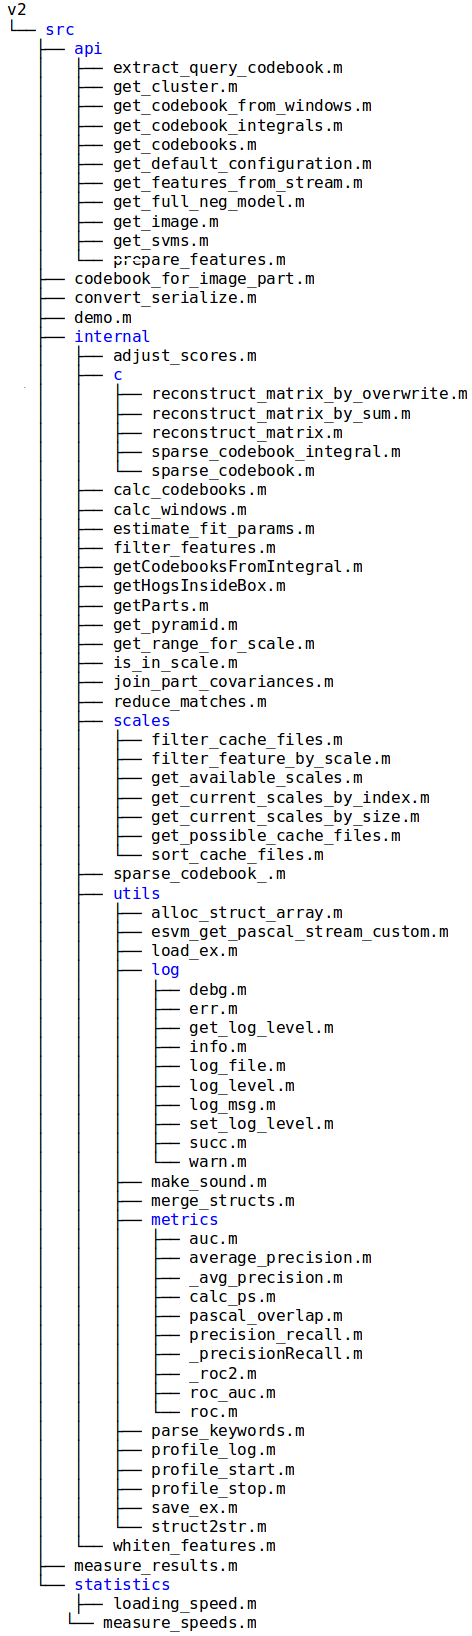
\includegraphics[width=\textwidth]{content/pictures/v2_full}
\caption{Filestructure of the framework}
\label{fig:v2_full}
\end{wrapfigure}

After the first experiments with the feature algorithms, codebook dimensions and \ac{SVM} usage were done, the second version of the framework was developed. The framework design was orientated on the ExemplarSVM framework. This means that some of the functions are reused as for example the parsing routines for a PASCAL dataset like \ac{VOC2011}. In contrast to the first version, no global variables are used (except for caching during automated tests). Instead all settings and temporary information is stored in a configuration structure which each function expect as its first argument. Besides of some ExemplarSVM settings used for the feature extraction, all parameters which affect the execution flow are defined as fields in the structure. The default settings as described in \prettyref{tab:configuration_framework} can be obtained by calling the \verb|get_default_configuration| function. Two utility functions for providing easy-to-use wrapper functions like the \verb|demo| function are \verb|parse_keywords| which allows to parse a list of arguments in a key value like fashion. In contrast to the \verb|inputParser| class from \MATLAB, a predefinition of the available arguments is not required (although they can be restricted according to a list of strings) and the \verb|merge_structs| function which merges multiple structs into a single struct. By combining the three functions, a simple configuration by using function arguments is implemented.

Similar to first version, every function which generates information from images contain routines to save and load data from a file based cache. The whole framework is designed to provide a transparent generation of data, saving and loading it from the cache. If the user calls such a function, it initially checks if a cache file exist at a file path constructed from the chosen configuration parameters. If available, the cache file will be loaded and returned. If not, it will try to generate the requested information by using the supplied arguments.


Most of the input and output values in the framework are structures or structure arrays. This provides the ability to access information on a per image base or getting an information of all images at once with a single line of code. Every time a higher amount of memory is required for arrays, its memory will be prealloctated if possible to reduce the overhead due to memory allocations and movement. For achieving this for structure arrays, a function \verb|alloc_struct_array| was implemented.

The \verb|demo| function represents a complete sample implementation using all modules from the framework. The function recognizes if it was run from a desktop or commandline (launched with the \textit{-nodesktop} option) instance of \MATLAB. If a desktop instance is used, the user will be asked interactively for a query image and afterwards to select a part from it to search for. If invoked from within a commandline instance the filename and bounding box is taken from the configuration structure.

The first step in the \verb|demo| function after a bounding box was selected is the creation of the query codebook. This is abstracted by the \verb|extract_query_codebook| function, which calculates the codebook from the image file or extracts it from the integral image for the query image. In the second step a \ac{SVM} is trained through the \verb|get_svms| function. If the calibration is enabled, the third step includes the calculation of sliding windows and corresponding codebooks for the query image and scoring them with the previously trained \ac{SVM}. A gaussian curve is afterwards fitted onto the scores and later used to adjust the scores obtained from the image database. The next step includes the loading of the corresponding database based on the size of the query part. When the database is loaded the currently computational most expensive part comes into play which calculates the sliding windows and extracts the codebooks from the integral images. For a speed up the work will be distributed over several pool workers. It had to be ensured that the data which has to be transfered between the workers and the main program is as small as possible. Tests showed that the parallization could even increase the computation time if the data required by the different workers becomes to large. Therefore it brings only a significant speed up if kd-Trees were used or the matrix reconstruction is done on the workers instead in the main program. The obtained codebooks are afterwards classified by the \ac{SVM}. If a calibration was used, all windows with scores above $-0.25$ are extracted from their source image and saved in the result folders. Without calibration, the first 100 windows after a non maximum suppression (sorted by decreasing scores) are saved. In addition a \textit{results.mat} file is also placed inside the folder. These files could be collected by the \verb|measure_results| function which calculates precision-recall curves and provide overviews about how the different parameter combinations behaved according to the ground truth from the \ac{VOC2011} dataset.
%TODO beschreibung der benutzung, image listen etc




\subsection{A modular approach}
